
\smallframetitle

\section{From 29/07/24 to 02/08/24}
\insertsectionframe


\subsection{Methodology for Identifying True Neighboring Base Stations Based on Antenna Azimuths}
\insertsubsectionframe

\begin{frame}
    \frametitle{Introduction: Challenges in Identifying True Neighboring Base Stations}

    \begin{block}{Key Challenges}
        \begin{itemize}
            \item \textbf{Wrong potential neighbors:} Delaunay triangulatio often fails to capture all potential neighbors, leading to incomplete graphs.
            \item \textbf{Azimuth Coverage:} Fixed beamwidths for antennas can result in inaccurate coverage areas, missing true neighboring connections.
            \item \textbf{Directional Alignment:} Even when stations are geometrically close, their azimuths may not be aligned, making them ineffective neighbors.
            \item \textbf{One-Way vs. Two-Way Connections:} Some stations may only be aligned in one direction, requiring a nuanced approach to capturing all meaningful relationships.
            \item \textbf{Edge Crossings:} In the process of graph construction, edge crossings can occur, complicating the interpretation of true neighboring relationships.
        \end{itemize}
    \end{block}

    \begin{block}{Objective}
        The following slides will discuss the methodologies developed to overcome these challenges, ensuring a more accurate and realistic representation of neighboring base stations in the network.
    \end{block}
\end{frame}


\begin{frame}
    \frametitle{Problem 1: Identifying Potential Neighbors Using kNN}

    \begin{block}{Overview}
        The initial problem was the identification of potential neighbors, where some of them might not be appropriate due to using a simple approach based on Delaunay triangulation, which only considers the geometric location of base stations.
    \end{block}

    \begin{block}{Solution}
        To address this, the k-Nearest Neighbors (kNN) approach was implemented, where each base station considers its closest \(K\) neighbors as potential connections. This method ensures that all relevant potential neighbors are included for further analysis.
    \end{block}

    \begin{block}{Methodology}
        \begin{itemize}
            \item \textbf{Set \(K\) Value:} Determine the number of neighbors \(K = 10\).
            \item \textbf{Construct kNN Graph}
            \item \textbf{Result:} A more inclusive set of potential neighbors, ready for further filtering based on azimuth and beamwidth data.
        \end{itemize}
    \end{block}
\end{frame}


\begin{frame}
    \frametitle{Problem 2: Calculating Accurate Beamwidths for Azimuths (Part 1)}
    \begin{columns}
        \begin{column}{0.5\textwidth}
    \begin{block}{Overview}
        The next issue was inaccurately defining the coverage areas for antennas based on fixed beamwidths, which could miss true neighboring connections.
    \end{block}
    \begin{block}{Solution}
        Dynamic beamwidth calculation tailored to the number of azimuths per base station. Special cases are handled for stations with only one or two azimuths.
    \end{block}
        \end{column}
        \begin{column}{0.5\textwidth}
            \begin{figure}
                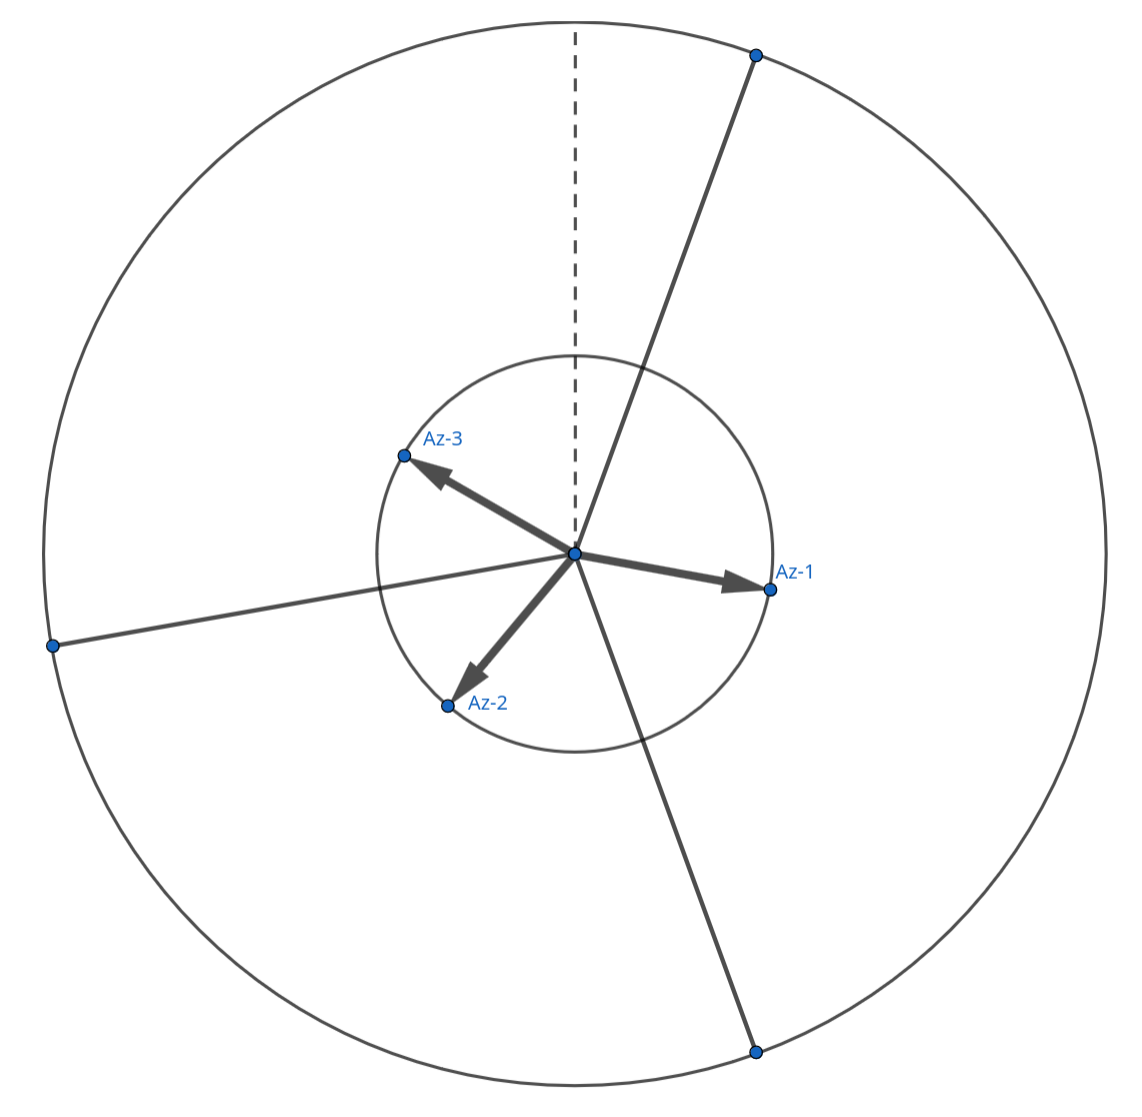
\includegraphics[width=0.7\textwidth]{images/Altair/az_beamwidth_calc.png}  
                \caption{Beamwidth calculation}
            \end{figure}
        \end{column}
    \end{columns}
\end{frame}

\begin{frame}
    \frametitle{Problem 2: Calculating Accurate Beamwidths for Azimuths (Part 2)}

    \begin{block}{Methodology}
        \begin{itemize}
            \item \textbf{Azimuth Sorting:} Begin by sorting the azimuth angles \( \alpha_1 < \alpha_2 < \dots < \alpha_n \).
            \item \textbf{Beamwidth Calculation:}
                \begin{itemize}
                    \item \textbf{Single Azimuth:} Assign a beamwidth of 180 degrees to cover the full semicircle.
                    \item \textbf{Two Azimuths:}
                        \begin{itemize}
                            \item Compute the angular difference between the two azimuths and assign each half of this difference as the beamwidth.
                            \item The remaining angle is allocated to complete the 360-degree coverage.
                        \end{itemize}
                    \item \textbf{Multiple Azimuths:}
                        \begin{itemize}
                            \item \textbf{Internal Azimuths:} 
                            \[
                            \Delta \alpha_{\text{bw}} = \frac{(\alpha_{i+1} - \alpha_i) + (\alpha_i - \alpha_{i-1})}{2}
                            \]
                            \item \textbf{First and Last Azimuths:} Special handling ensures circular coverage:
                            \begin{align*}
                            \Delta \alpha_{\text{bw}} & = \frac{(\alpha_2 - \alpha_1) + (360 - \alpha_n + \alpha_1)}{2} & \Delta \alpha_{\text{bw}} & = \frac{(\alpha_1 + 360 - \alpha_n) + (\alpha_n - \alpha_{n-1})}{2}
                            \end{align*}
                        \end{itemize}
                \end{itemize}
            \item \textbf{Result:} Accurate coverage angles for each azimuth, leading to better identification of true neighboring stations.
        \end{itemize}
    \end{block}
\end{frame}

\begin{frame}
    \frametitle{Problem 3: Calculating Direction Coefficient and Identifying Real Neighbors (Part 1)}

    \begin{block}{Overview}
        The challenge was not only to determine physical proximity but also to assess how well the azimuths of neighboring base stations were aligned. To achieve this, we needed a robust metric to quantify this alignment and ensure that only truly aligned neighbors were considered valid connections.
    \end{block}

    \begin{block}{Solution}
        We introduced the \textbf{Direction Coefficient} \( \alpha \), ranging from 0 to 1, to quantify the alignment between the azimuth of a base station and the direction to its neighbor. An \( \alpha \) value of 1 indicates perfect alignment, while a value of 0 indicates no alignment.
    \end{block}
\end{frame}

\begin{frame}
    \frametitle{Problem 3: Calculating Direction Coefficient and Identifying Real Neighbors (Part 2)}

    \begin{block}{Methodology}
        \begin{itemize}
            \item \textbf{Direction Calculation:}
            \begin{itemize}
                \item Calculate the direction vector from the base station to its potential neighbor.
                \item Convert this vector into an angle \( \theta \) in degrees using arctangent, ensuring it falls within [0, 360) degrees.
            \end{itemize}
            \item \textbf{Beamwidth Check:}
            \begin{itemize}
                \item Determine the range defined by the azimuth's beamwidth.
                \item Check if the calculated direction angle \( \theta \) falls within this range.
                \item Proceed to calculate \( \alpha \) if the direction is within the beamwidth.
            \end{itemize}
            \item \textbf{Angle Difference Calculation:}
            \begin{itemize}
                \item Calculate the angular difference between the azimuth and the direction angle \( \theta \).
                \item Use the smallest angular difference (either direct or complementary) for accurate alignment measurement.
                \item **Note:** If the angle difference exceeds 90 degrees, set \( \alpha = 0 \), indicating the directions are not aligned.
            \end{itemize}
        \end{itemize}
    \end{block}
\end{frame}

\begin{frame}
    \frametitle{Problem 3: Calculating Direction Coefficient and Identifying Real Neighbors (Part 3)}

    \begin{block}{Methodology (cont.)}
        \begin{itemize}
            \item \textbf{Cosine Similarity Calculation:}
            \begin{itemize}
                \item Represent both the azimuth and the direction as vectors in a 2D plane.
                \item Calculate the cosine of the angle between these vectors to measure alignment.
            \end{itemize}
            \item \textbf{Normalization to \( \alpha \):}
            \begin{itemize}
                \item Normalize the cosine similarity to a range of [0, 1] using the formula \( \alpha = \frac{1 + \cos(\text{angle difference})}{2} \).
                \item A higher \( \alpha \) indicates better alignment between the azimuth and the direction.
            \end{itemize}
            \item \textbf{Final Neighbor Validation:}
            \begin{itemize}
                \item Connections with \( \alpha \) values exceeding the predefined threshold are retained as real neighbors.
                \item This approach ensures that only well-aligned stations are considered as neighbors, improving the accuracy and realism of the graph.
            \end{itemize}
        \end{itemize}
    \end{block}
\end{frame}

\begin{frame}
    \frametitle{Problem 4: Handling One-Way Neighboring Stations}

    \begin{block}{Overview}
        Initially, only stations with mutual (bi-directional) azimuth alignment were considered as neighbors. However, this approach excluded valid connections where alignment was only one-way. It was essential to adjust the methodology to capture these one-way alignments to accurately represent the network.
    \end{block}

    \begin{block}{Solution}
        The methodology was enhanced to consider one-way alignments. If at least one station's azimuth covers the neighboring station within its beamwidth, the connection is considered valid, even if there is no reverse alignment.
    \end{block}
\end{frame}

\begin{frame}
    \frametitle{Problem 4: Handling One-Way Neighboring Stations (Cont.)}

    \begin{block}{Methodology}
        \begin{itemize}
            \item \textbf{Bi-Directional Alignment Check:}
            \begin{itemize}
                \item For each base station, verify if the neighboring station is within the beamwidth of its azimuth and vice versa.
                \item Calculate \( \alpha \) for both directions. If both are sufficiently high, retain the connection.
            \end{itemize}
            \item \textbf{One-Way Alignment Check:}
            \begin{itemize}
                \item If no bi-directional alignment is found, check if at least one station's azimuth covers the other.
                \item Apply the \( \alpha \) coefficient to this one-way alignment; if \( \alpha \) exceeds the threshold, the connection is retained.
            \end{itemize}
            \item \textbf{Unified Neighbor Validation:}
            \begin{itemize}
                \item Both bi-directional and one-way connections are validated using the \( \alpha \) coefficient.
                \item This approach ensures that the graph accurately reflects all meaningful connections, whether one-way or two-way.
            \end{itemize}
        \end{itemize}
    \end{block}
\end{frame}


\begin{frame}
    \frametitle{Problem 5: Edge Crossing in Neighboring Graph}

    \begin{block}{Problem Overview}
        During the construction of the neighboring graph for cellular base stations, we encountered a problem where edges (connections) between base stations were crossing each other. This could lead to incorrect conclusions about which stations are truly neighboring.
    \end{block}
    \begin{columns}
        \begin{column}{0.5\textwidth}
            \begin{block}{Approach Overview}
                To solve the edge crossing problem, we employed the following methodological approach:
                \begin{itemize}
                    \item Sort edges by length.
                    \item Sequentially add edges to the graph.
                    \item Check for intersections with already added edges.
                    \item Exclude intersecting edges.
                    \item Construct a final graph without crossings.
                \end{itemize}
            \end{block}
        \end{column}
        \begin{column}{0.5\textwidth}
            \begin{figure}
                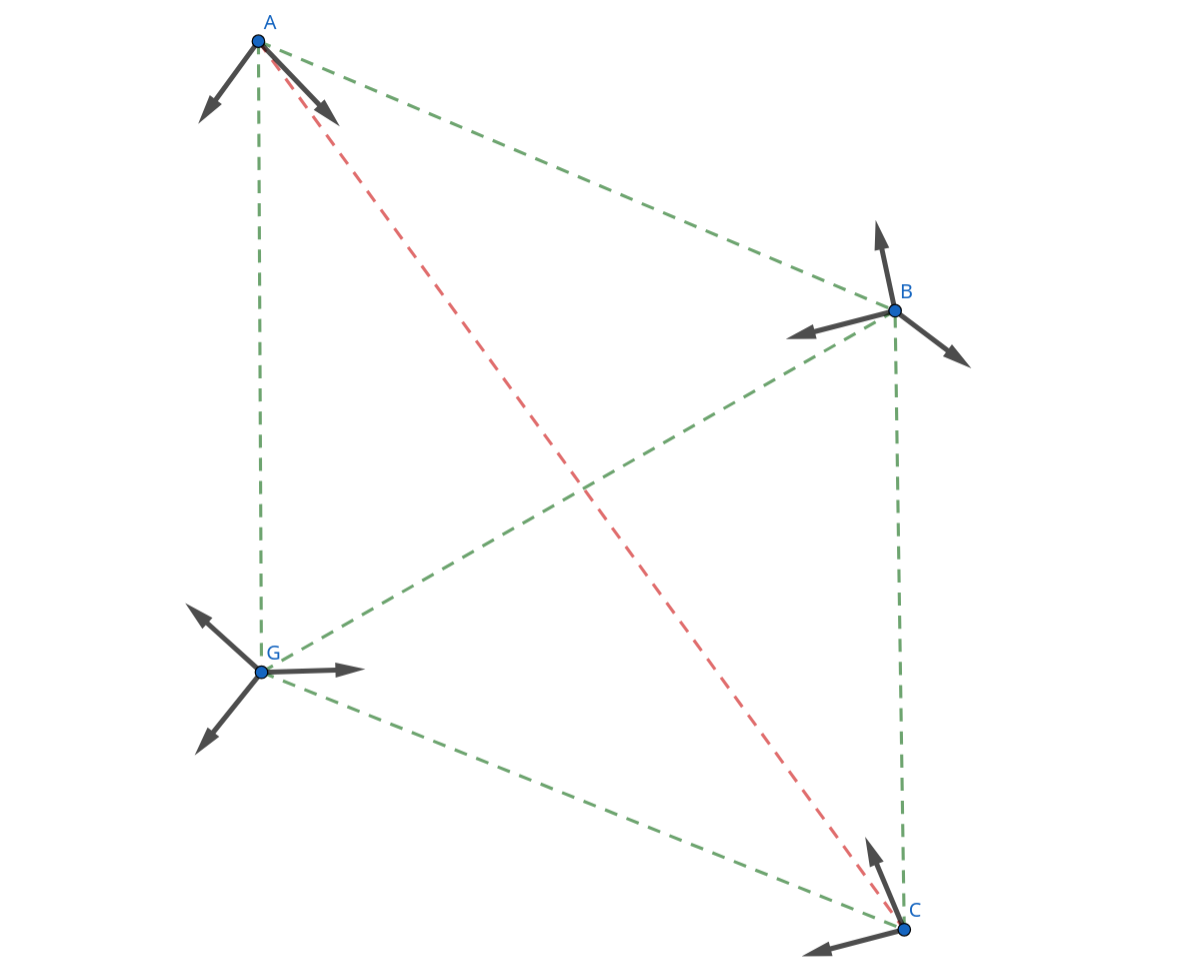
\includegraphics[width=0.5\textwidth]{images/Altair/edge_crossing_problem.png}  
                \caption{Edge Crossing problem}
            \end{figure}
        \end{column}
    \end{columns}
\end{frame}



